%%% Local Variables:
%%% mode: latex
%%% TeX-master: "<none>"
%%% End:

\title{Motion Compensated Discrete Wavelet Transform (MCDWT)}

\author{Vicente González Ruiz}

\maketitle
\tableofcontents

\section{Intro}

\href{https://en.wikipedia.org/wiki/Video}{Video} data contain high
amounts of redundancy, spatial and temporal. For this reason, most of
video encoders compress the input sequece of images (which are
matrices of \href{https://en.wikipedia.org/wiki/Pixel}{pixels})
basically in two stages: (1) a transform stage in the
\href{https://en.wikipedia.org/wiki/Time_domain}{time} and in the
\href{https://www.quora.com/What-is-spatial-domain-in-image-processing}{spatial}
domains that produces a collection of spatially
\href{https://en.wikipedia.org/wiki/Decorrelation}{uncorrelated}
\href{https://www.quora.com/What-is-spatial-domain-in-image-processing}{coefficients},
and (2) an
\href{https://vicente-gonzalez-ruiz.github.io/symbol_compression/}{entropy
  encoding} phase to remove the statistical redundancy that still can
remains after the decorrelation (transform). These coefficients have
two interesting features:
\begin{itemize}
\item Usually, a \textbf{smaller entropy} than the original
  pixels. This helps to increase the compression ratios.
\item The transform domain provides a
  \textbf{\href{https://en.wikipedia.org/wiki/Image_resolution}{multiresolution}
    representation} of the visual information (spatial
  \href{http://inst.eecs.berkeley.edu/~ee290t/sp04/lectures/videowavelet_UCB1-3.pdf}{scalability}).
\end{itemize}

\section{Distrete Wavelet Transform (DWT)}
\href{https://en.wikipedia.org/wiki/Discrete_wavelet_transform}{(2D-)DWT}
applied to an image is a suitable transform for obtaining a spatial
(2D) decorrelation and, at the same time, a
\href{https://vicente-gonzalez-ruiz.github.io/image_transformations_for_coding/indexse24.html#x34-3400024}{multiresolution
  dyadic representation} of such image, conforming a collection of DWT
subbands. The forward transform converts the image into a set of
frequency subbands with coefficients representing different spatial
areas and frequency orientations. There is a equivalence between (DWT)
subbands (a \emph{(subband) decomposition}) and
\href{https://en.wikipedia.org/wiki/Pyramid_(image_processing)#Laplacian_pyramid}{Lapacian
  pyramids}, and it is quite simple to pass from a
\href{https://vicente-gonzalez-ruiz.github.io/pyramids-and-wavelets/}{a
  decomposition representation to a pyramid representation and
  viceversa}.

\href{https://github.com/vicente-gonzalez-ruiz/MCDWT/blob/master/src/DWT.py}{DWT.py}
implements the forward and backward (2D-)DWT for color images. $L$ and
$H$ stands for \emph{low-pass filtered} and \emph{high-pass filtered},
respectively.  More information about the implementation can be found at
\href{https://pywavelets.readthedocs.io/en/latest/index.html}{PyWavelets}.

\lstinputlisting[firstline=9, lastline=130, language=python, caption=DWT.py]{../src/DWT.py}

The multilevel DWT is a recursive use of the (1-level) DWT applied to
the $LL$ subband. For example, if the DWT is applied $k$-times to the
$LL$ subband, recursively, a decomposition of $k+1$-levels is generated. For
the sake of simplicity, we will denote the subbands $\{LH^k, HL^k,
HH^k\}$ as only $H^k$, and $LL^k$ as only $L^k$.

\subsection{Scalability provided by DWT}
Depending on the DWT subbands (pyramid levels in the pyramid
representation) that we use, we can reconstruct a image at different
spatial at scales (resolutions). For example, the scale $2$ of an
image $s_1$ that has been transformed using the DWT of 2 levels will
be represented by the subband $s_1.L^2$, the scale $1$ by the subband
$s_1.L=\text{iDWT}(s_1.L^2, S_1.H^2)$, and the scale $0$ (the original
resolution of the image) by the subband $s_1.L^0=\text{iDWT}(s_1.L,
s_1.H)$.

\section{Motion DWT (MDWT)}
DWT can be applied to a sequence of images by simply transforming each
image of the sequence independently. This is done, for example, in the
\href{https://en.wikipedia.org/wiki/JPEG_2000}{motion JPEG2000 video
  compression standard}. Notice that only the spatial redundancy is
exploited. All the temporal redundancy still remains in the video.

\begin{figure}
\centering
\imgw{400}{graphics/forward_MDWT.svg}
\caption{Forward MDWT step.}
\end{figure}

\lstinputlisting[firstline=16, lastline=62, language=python, caption=MDWT.py]{../src/MDWT.py}

\subsection{Scalability provided by MDWT}
MDWT sequences (of (subband) decompositions) are scalable in space and
in time. Spatial scalability is a direct consequence of DWT. On the other
hand, it is trivial to observe that MDWT provides \emph{fully}
temporal scalability (we can access to the images randomly) because
each image of the input sequence is transformed independently.

\section{Video transform alternatives}
To remove both, spatial and temporal redundancies, two different
alternatives are available: (1) a t+2D transform or (2) a 2D+t
transform. In a t+2D transform, the video is first
\href{https://en.wikipedia.org/wiki/Digital_filter\#Analysis_techniques}{analyzed} (transformed)
over the time domain and next, over the space domain. A 2D+t transform
does just the opposite.

Each choice has a number of \emph{pros} and \emph{cons}. For example,
in a t+2D transform we can apply directly any image predictor based on
motion estimation because the input is a normal video. However, if we
implement a 2D+t transform, the input to the motion estimator is a
sequence decompositions.
\href{http://www.polyvalens.com/blog/wavelets/theory}{The overwhelming
  majority of DWT's} are not
\href{http://www.polyvalens.com/blog/wavelets/theory}{shift
  invariant}, which basically means $\text{DWT}(s[t]) \neq
\text{DWT}(s[t+x])$, where $x$ is a displacement of $s[t]$ along the
time domain.  Therefore, motion estimators which compare pixel values
will not work on the (subband) decomposition domain. On the other
hand, if we want to provide true spatial scalability (processing only
those
\href{https://en.wikipedia.org/wiki/Image_resolution\#Spatial_resolution}{spatial
  resolutions} (scales) necessary to get a spatially scaled of our
video), a t+2D transformed video is not suitable because the first
step of the forward transform (t) should be reversed at full
resolution in the backward transform (as the forward transform did).

\section{Motion Compensated Discrete Wavelet Transform (MCDWT)}
MCDWT is a 2D+t transform. The 2D stage is MDWT. The t stage is a
1D-DWT, which removes the temporal redundancy between adjacent $H$
subbands by means of
\href{https://en.wikipedia.org/wiki/Motion_compensation}{Motion
  Compensation (MC)}. A special characteristic of MCDWT is that the
motion information is not transmitted from the encoder to the
\href{https://en.wikipedia.org/wiki/Decoder}{decoder}. This is possible because to estimate de motion at the
encoder, it only uses the information that it is accesible by the
decoder.

\subsection{MCDWT butterfly}

MCDWT butterly inputs three decompositions $a=\{a.L, a.H\}$, $b=\{b.L,
b.H\}$ and $c=\{c.L, c.H\}$, and outputs a residue subband
$\tilde{b}.H$, which replaces to $b.H$ in the original $b$
pyramid. So, after the use of the bufferfly, we get $a=\{a.L, a.H\}$
(an intra-coded ``I'' image), $\tilde{b}=\{b.L, \tilde{b}.H\}$ (a
bidirectionally predicted ``B'' image) and $c=\{c.L, c.H\}$ (an
intra-coded ``I'' image). Obviously, this replacement is fully
reversible. Notice that the
\href{http://www.vtvt.ece.vt.edu/research/references/video/DCT_Video_Compression/Zhang92a.pdf}{pyramid
  domain} (which is invariant to the pixels displacements) has been
used to estimate and compensate the $H$ subbands (levels of the
corresponding pyramid).

\begin{figure}
\centering
\imgw{800}{graphics/forward_butterfly.svg}
\caption{Forward MCDWT butterfly.}
\end{figure}
\lstinputlisting[firstline=20, lastline=67, language=python, caption=MCDWT.py]{../src/MCDWT.py}

Notice that, even if $a$ and $c$ (at full resolution) are available at
the decoder, only $b.L$ is. So, it does not make sense to search the
low resolution structures of $b.L$ in the high resolution images $a$
and $c$, because even if a perfect match is achieved (think about the
tree images $a$, $b$ and $c$ are identical), the prediction error
would be different than $0$ as a consequence of that the high
resolution information is missing in $b.L$.

\subsection{MCDWT forward transform}

The MCDWT forward transform is the result of appliying the MCDWT
butterfly to all the input sequence of pyramids with different
distances between the decompositions. As a consequence, except the
first and the last $H$-subband of the sequence are temporally
decorrelated.

\begin{figure}
\centering
\imgw{800}{graphics/temporal_decorrelation.svg}
\caption{MCDWT forward transform.\label{fig:forward_MCDWT}}
\end{figure}
\lstinputlisting[firstline=69, lastline=138, language=python, caption=MCDWT.py]{../src/MCDWT.py}

\subsection{Scalability provided by MCDWT}
The decomposition generated by the MCDWT is identical to
MDWT. Therefore, MCDWT provides the same spatial scalability than
MDWT. In order to obtain several spatial resolutions, MCDWT should be
applied to the low-frequency subbands, recursively. As an example, in
the Figure~\ref{fig:multiresolution}, MCDWT has been applied to the
output of the example of the Figure~\ref{fig:forward_MCDWT}. Notice
that between two consecutive iterations of MCDWT, MDWT must be applied
to the low-frequency subband in order to reduce the resolution of the
analysis.

On the other hand, MCDWT decreases the temporal scalability offered by
MDWT to allowing only dyadic access (depending on required image and
the number of MCDWT levels, more than one decomposition need to be
inversely transformed). For example, if only one step of the backward
transform is applied to the previous example, only the decompositions
of $s_0$, $s_2$ and $s_4$ will be reconstructed (the first
\href{https://en.wikipedia.org/wiki/Temporal_resolution}{temporal
  resolution}. If a second iteration of the backward transform is
used, all the pyramids are rendered.

\begin{figure}
\centering
\imgw{800}{graphics/multiresolution.svg}
\caption{MDWT+MCDWT multiresolution procedure.\label{fig:multiresolution}}
\end{figure}

\begin{comment}
\end{document}

\section{Video \href{http://inst.eecs.berkeley.edu/~ee290t/sp04/lectures/videowavelet_UCB1-3.pdf}{scalability}}
MCDWT inputs a \href{https://en.wikipedia.org/wiki/Video}{video} (a
sequence of images) and outputs a video (a sequece of pyramids), in
such a way that when only a portion of the data of the transformed
video is used, a video with a lower
\href{https://en.wikipedia.org/wiki/Temporal_resolution}{temporal
resolution}, lower
\href{https://en.wikipedia.org/wiki/Image_resolution\#Spatial_resolution}{spatial
resolution} or/and lower
\href{https://en.wikipedia.org/wiki/Compression_artifact}{quality} can
be generated.

If all the transformed data is used, then the original video is
restored (MCDWT is a lossless transform). The forward transform's
output has exactly the same number of pyramids than images are in the
input video (for example, no extra motion fields are produced). At
this time, we will focuse only on spatial
\href{http://inst.eecs.berkeley.edu/~ee290t/sp04/lectures/videowavelet_UCB1-3.pdf}{scalability}. Window Of Interest (WOI) and quality scabilities will be addressed later.



\subsection{Another example (only butterfly)}
Lets suppose that we have procesed the sequence of images one step and a
second one is performed on the output of this first step. At this
moment, the structure of the images would be:

\subsubsection{Analyze the input images}
\begin{equation}
  \{A.L^2, A.H^2\} = \text{DWT}(A.L)\\
  \{B.L^2, B.H^2\} = \text{DWT}(B.L)\\
  \{C.L^2, C.H^2\} = \text{DWT}(C.L)
\end{equation}

\subsubsection{Zoom-in $L$ subbands}{Zoom-in L subbands}
\begin{equation}
  [A.L^2] = \text{iDWT}(A.L^2, 0)\\
  [B.L^2] = \text{iDWT}(B.L^2, 0)\\
  [C.L^2] = \text{iDWT}(C.L^2, 0)
\end{equation}

\subsubsection{Merge and zoom-in $H$ subbands
\begin{equation}
  [A.H^2] = \text{iDWT}(0, A.H^2)\\
  [B.H^2] = \text{iDWT}(0, B.H^2)\\
  [C.H^2] = \text{iDWT}(0, C.H^2)
\end{equation}

\subsubsection{Generate a prediction $[\hat{B}.H^2]$¡}
\begin{equation}
  [B_A.H^2] = [A.H^2]\overset{[A.L^2]\rightarrow[B.L^2]}{\longrightarrow}[B.H^2]\\
  [B_C.H^2] = [C.H^2]\overset{[C.L^2]\rightarrow[B.L^2]}{\longrightarrow}[B.H^2]\\  
\end{equation}

Note: predictions do not need to be exhaustive. Depending on the quality
of the predictions for $[B.L^2]$:

\begin{equation}
  [B_A.L^2] = [A.L^2]\overset{[A.L^2]\rightarrow[B.L^2]}{\longrightarrow}[B.L^2]\\
  [B_C.L^2] = [C.L^2]\overset{[C.L^2]\rightarrow[B.L^2]}{\longrightarrow}[B.L^2],\\  
\end{equation}

comparing $[B_A.L^2]$ and $[B_C.L^2]$ with $[B.L^2]$. In fact,
$[B_A.H^2]$ and $[B_C.H^2]$ could have ``holes'' (regions to 0,
supposing that the pixels are positive), producing a parcial prediction
$[\hat{B}.H^2]$ for $[B.H^2]$. In the simplest case

\begin{equation}
  [\hat{B}.H^2] = \frac{[B_A.H^2] + [B_C.H^2]}{2}.
\end{equation}

Finally, (as in the forward transform) the prediction should take into
cosideration how to minimize the energy of the residue

\begin{equation}
  [\tilde{B}.L^2] = [B.L^2] - [\hat{B}.L^2].
\end{equation}

\subsubsection{Compute the residue $[\tilde{B}.H^2]$}
\begin{equation}
  [\tilde{B}.H^2] = [B.H^2] - [\hat{B}.H^2]
\end{equation}

\subsubsection{Unmerge $\tilde{B}.H^2$ subbands}
\begin{equation}
  \tilde{B}.H^2 = \text{DWT}(0, [\tilde{B}.H^2])
\end{equation}

\hypertarget{compose-the-residue-in-the-wavelet-domain}{%
\subsubsection{Compose the residue in the wavelet
domain}\label{compose-the-residue-in-the-wavelet-domain}}

\begin{equation}
   \{B.L^2, \tilde{B}.H^2\}
\end{equation}

\section{8. Backward (inverse) MCDWT butterfly}
\subsection{Input}
\begin{itemize}
\tightlist
\item
  Three frames $A=\{A.L, A.H\}$, $B=\{B.L, \tilde{B}.H\}$, and
  $C=\{C.L, C.H\}$.
\end{itemize}

\subsection{Output}
\begin{itemize}
\tightlist
\item
  Three frames $a$, $b$ and $c$.
\end{itemize}

\subsection{Algorithm}
\begin{figure}
\centering
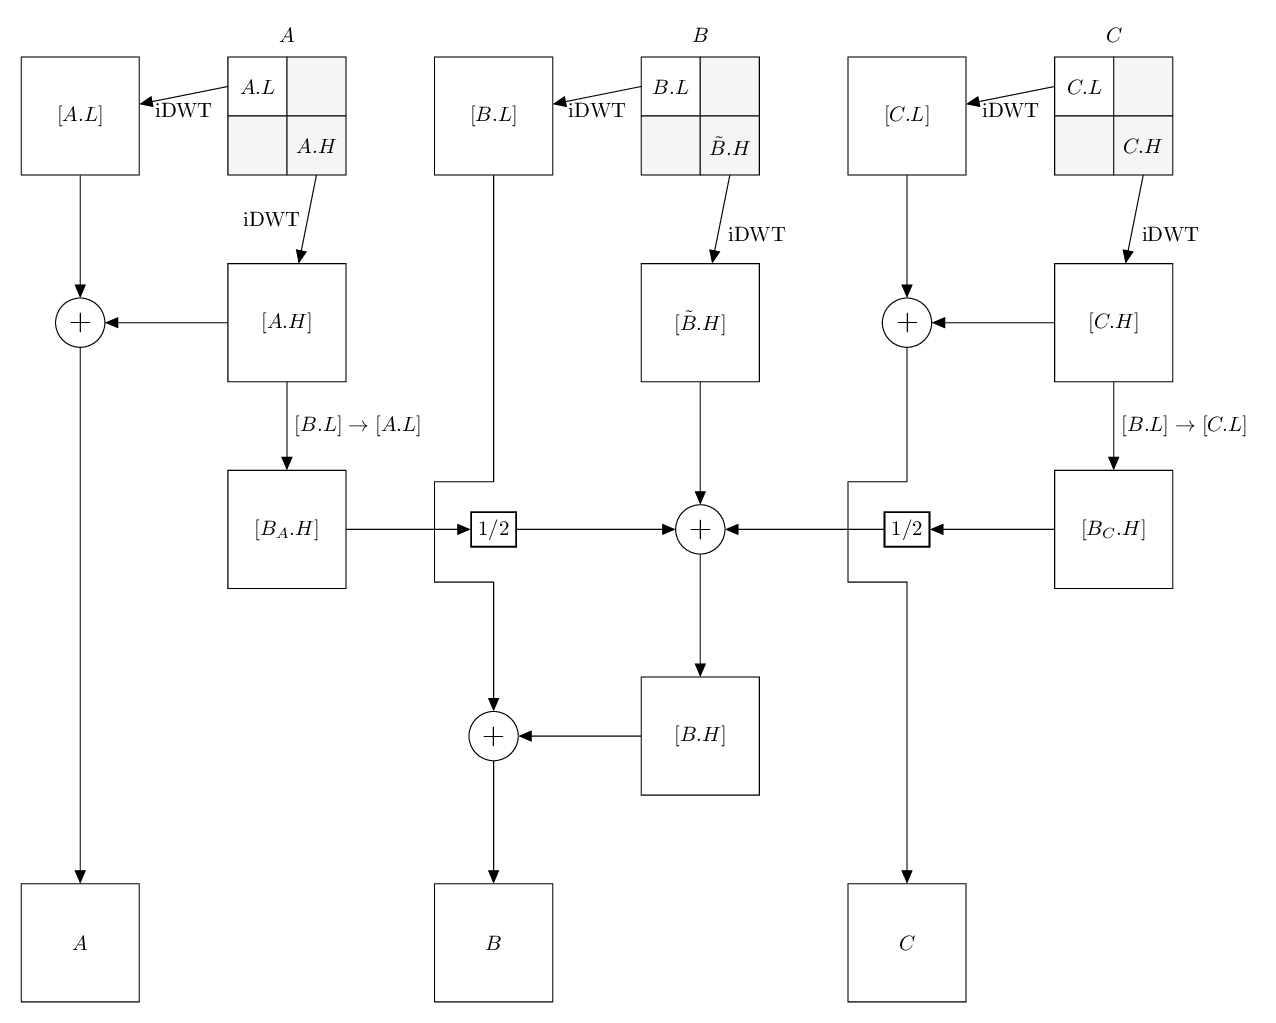
\includegraphics{backward.png}
\caption{MCDWT}
\end{figure}

\subsection{Example continuation (only one butterfly)}
Lets restore the structure for the three transformed images of
Section \ref{another_example}.

\subsubsection{Zoom-in $L$ subbands}
\begin{equation}
  [A.L^2] = \text{iDWT}(A.L^2, 0)\\
  [B.L^2] = \text{iDWT}(B.L^2, 0)\\
  [C.L^2] = \text{iDWT}(C.L^2, 0)
\end{equation}

\subsubsection{Merge (and zoom-in) $H$ subbands}
\begin{equation}
  [A.H^2] = \text{iDWT}(0, A.H^2)\\
  [\tilde{B}.H^2] = \text{iDWT}(0, \tilde{B}.H^2)\\
  [C.H^2] = \text{iDWT}(0, C.H^2)
\end{equation}

\subsubsection{Generate a prediction $[\hat{B}.H^2]$}
Identical to the prediction step performed at the forward transform.

\subsubsection{Restore the original subband $[B.H^2]$}
\begin{equation}
  [B.H^2] = [\hat{B}.H^2] + [\tilde{B}.H^2]
\end{equation}

\subsubsection{Compute $L$ subbands}
\begin{equation}
  A.L = [A.L^2] + [A.H^2]\\
  B.L = [B.L^2] + [B.H^2]\\
  C.L = [C.L^2] + [C.H^2]
\end{equation}

\subsection{$K$-levels (forward) MCDWT}
\subsubsection{Input}
\begin{itemize}
\tightlist
\item
  A sequence $s$ of $N$ images.
\end{itemize}

\subsubsection{Output}
\begin{itemize}
\tightlist
\item
  A sequence of $K+1$ temporal subbands, where each subband is a
  sequence of $N/2^K$ (wavelet) pyramids.
\end{itemize}

\subsubsection{Algorithm}

\subsubsection{Data extraction examples}
\paragraph{Temporal scalability}
\begin{itemize}
\item
  Scale 2:

  \$ s\_0.L\^{}0 = \text{DWT}\^{}\{-2\}(S\_0) =
  \text{DWT}\textsuperscript{\{-1\}(\text{DWT}}\{-1\}(s\_0.L\^{}2,
  s\_0.H\^{}2), s\_0.H\textsuperscript{1),\textbackslash{} s\_4.L}0 =
  \text{DWT}\textsuperscript{\{-2\}(S\_4),\textbackslash{} s\_2.L}0 =
  \text{MCDWT}\^{}\{-2\}(S\_0, S\_2, S\_4) = (s\_2.L\^{}1 =
  \text{MCDWT}\textsuperscript{\{-1\}(\{s\_0.L}2,s\_0.H\^{}2\},
  \{s\_4.L\^{}2, s\_4.H\^{}2\}, \{s\_2.L\^{}2, \tilde{s}\_2.H\^{}2\}))
  \$
\end{itemize}

\paragraph{Spatial scalability}
\begin{itemize}
\item
  Scale 2:

  \$ s\_0.L\^{}2, s\_1.L\^{}2, s\_2.L\^{}2, s\_3.L\^{}2, s\_3.L\^{}2. \$
\item
  Scale 1:

  \$ s\_0.L\^{}1 = DWT\textsuperscript{\{-1\}(s\_0.L}2, s\_0,H\^{}2),
  \textbackslash{} s\_4.L\^{}1 = DWT\textsuperscript{\{-1\}(s\_4.L}2,
  s\_4.H\^{}2), \textbackslash{} s\_2.L\^{}1 =
  MCDWT\textsuperscript{\{-1\}(s\_0.L}1, s\_2.L\^{}2, s\_4.L\^{}1),
  \textbackslash{} s\_1.L\^{}1 = MCDWT\textsuperscript{\{-1\}(s\_0.L}1,
  s\_1.L\^{}2, s\_2.L\^{}1), \textbackslash{} s\_3.L\^{}1 =
  MCDWT\textsuperscript{\{-1\}(s\_2.L}1, s\_3.L\^{}2, s\_4.L\^{}1). \$
\item
  Scale 0:

  \$ s\_0.L\^{}0 = DWT\textsuperscript{\{-1\}(s\_0.L}1,
  s\_0.H\textsuperscript{1),\textbackslash{} s\_4.L}0 =
  DWT\textsuperscript{\{-1\}(s\_4.L}1, s\_4.H`1),\textbackslash{}
  s\_2.L\^{}0 = MCDWT\textsuperscript{\{-1\}(s\_0.L}0, s\_2.L\^{}1,
  s\_4.L\textsuperscript{0),\textbackslash{} s\_1.L}0 =
  MCDWT\textsuperscript{\{-1\}(s\_0.L}0, s\_1.L\^{}1,
  s\_2.L\textsuperscript{0),\textbackslash{} s\_3.L}0 =
  MCDWT\textsuperscript{\{-1\}(s\_2.L}0, s\_3.L\^{}2, s\_4.L\^{}0). \$
\end{itemize}

    Provided by the execution of iMCDWT.

\begin{enumerate}
\def\labelenumi{\arabic{enumi}.}
\tightlist
\item
  Scale 2:
\end{enumerate}

Provided by subbands \texttt{L} of the pyramids. We don't need to carry
out any computation.

\begin{enumerate}
\def\labelenumi{\arabic{enumi}.}
\setcounter{enumi}{1}
\tightlist
\item
  Scale 1:
\end{enumerate}

Rendered after running iMCDWT one iteration. For 3 pyramids
\texttt{A=\{A.L,A.H\}}, \texttt{B=\{B.L,\textasciitilde{}B.H\}} and
\texttt{C=\{C.L,C.H\}} where the subband \texttt{L} is the scale 2, the
scale 1 is recostructed by (see Algorithm iMCDWT\_step):

\begin{Shaded}
\begin{Highlighting}[]
\NormalTok{  x }\OperatorTok{=} \DecValTok{2}\OperatorTok{**}\DecValTok{2} \OperatorTok{=} \DecValTok{4}
\NormalTok{  [A.L] }\OperatorTok{=}\NormalTok{ 2D_iDWT(A.L,}\DecValTok{0}\NormalTok{)}\OperatorTok{;}                              \OperatorTok{>}\NormalTok{ Interpolate low}\OperatorTok{-}\NormalTok{freqs A.L of V[}\DecValTok{0}\NormalTok{]}
\NormalTok{  [A.H] }\OperatorTok{=}\NormalTok{ 2D_iDWT(}\DecValTok{0}\NormalTok{,A.H)}\OperatorTok{;}                              \OperatorTok{>}\NormalTok{ Interpolate high}\OperatorTok{-}\NormalTok{freqs A.H of V[}\DecValTok{0}\NormalTok{]}
\NormalTok{  V[}\DecValTok{0}\NormalTok{] }\OperatorTok{=}\NormalTok{ [A.L] }\OperatorTok{+}\NormalTok{ [A.H]}\OperatorTok{;}                                \OperatorTok{>}\NormalTok{ Reconstruct V[}\DecValTok{0}\NormalTok{] at spatial level }\DecValTok{1}
\NormalTok{  [B.L] }\OperatorTok{=}\NormalTok{ 2D_iDWT(V[}\DecValTok{1}\NormalTok{].L,}\DecValTok{0}\NormalTok{)}\OperatorTok{;}                           \OperatorTok{>} 
\NormalTok{  [}\OperatorTok{~}\NormalTok{B.H] }\OperatorTok{=}\NormalTok{ 2D_iDWT(}\DecValTok{0}\NormalTok{,V[}\DecValTok{1}\NormalTok{].H)}\OperatorTok{;}
\NormalTok{  [C.L] }\OperatorTok{=}\NormalTok{ 2D_iDWT(V[}\DecValTok{2}\NormalTok{].L,}\DecValTok{0}\NormalTok{)}\OperatorTok{;}
\NormalTok{  [C.H] }\OperatorTok{=}\NormalTok{ 2D_iDWT(}\DecValTok{0}\NormalTok{,V[}\DecValTok{2}\NormalTok{].H)}\OperatorTok{;}
\NormalTok{  V[}\DecValTok{2}\NormalTok{] }\OperatorTok{=}\NormalTok{ [C.L] }\OperatorTok{+}\NormalTok{ [C.H] }
\NormalTok{  [B.L]}\OperatorTok{->}\NormalTok{[A.L] }\OperatorTok{=}\NormalTok{ ME([B.L], [A.L])}
\NormalTok{  [B.L]}\OperatorTok{->}\NormalTok{[C.L] }\OperatorTok{=}\NormalTok{ ME([B.L], [C.L])}
\NormalTok{  [B.H]_A }\OperatorTok{=}\NormalTok{ MC([A.H], [B.L]}\OperatorTok{->}\NormalTok{[A.L])}
\NormalTok{  [B.H]_C }\OperatorTok{=}\NormalTok{ MC([C.H], [B.L]}\OperatorTok{->}\NormalTok{[C.L])}
\NormalTok{  [B.H] }\OperatorTok{=}\NormalTok{ [}\OperatorTok{~}\NormalTok{B.H] }\OperatorTok{+} \BuiltInTok{int}\NormalTok{(}\BuiltInTok{round}\NormalTok{(([B.H]_A }\OperatorTok{+}\NormalTok{ [B.H]_C)}\OperatorTok{/}\FloatTok{2.0}\NormalTok{))}
\NormalTok{  V[}\DecValTok{1}\NormalTok{] }\OperatorTok{=}\NormalTok{ [B.L] }\OperatorTok{+}\NormalTok{ [B.H]}
\NormalTok{  [A.L] }\OperatorTok{=}\NormalTok{ [C.L]}
\NormalTok{  [A.H] }\OperatorTok{=}\NormalTok{ [C.H]}
\end{Highlighting}
\end{Shaded}

\begin{enumerate}
\def\labelenumi{\arabic{enumi}.}
\setcounter{enumi}{2}
\tightlist
\item
  Scale 0:
\end{enumerate}

Repeat the previous computations.

\begin{enumerate}
\def\labelenumi{\arabic{enumi}.}
\setcounter{enumi}{3}
\tightlist
\item
  Scale -1:
\end{enumerate}

Repeat the previous computations, placing 0's in the H subbands.

\section{Temporal scalability}
Provided by the pruned execution of iMCDWT. Depending on the index of
the image to render, a number of images, that ranges between
:math:\texttt{1} (the best case) and :math:\texttt{1+l} (the worst
case), are decoded.

\section{Quality scalability}
Provided by partially reconstructing a set of coefficients selected by
their contribution to the minimization of the distortion.

    A sequence \texttt{S} of \texttt{N} (wavelet) pyramids, organized in
\texttt{T} temporal subbands, where each temporal subband is a sequence
of spatial pyramids. The number of input and output pyramids is the
same.

For example, if \texttt{l=2} and \texttt{n=5}:

\begin{verbatim}
      Spatial
      scale 0 1 2       t = 1                               t = 3
            ^ ^ ^ +---+---+-------+                   +---+---+-------+                                ^
            | | | |   |   |       |                   |   |   |       |                                |
            | | v +---+---+       |                   +---+---+    O <---- T[3][y][x]                  |
            | |   |   |   |       |                   |   |   |       |                                |
            | v   +---+---+-------+                   +---+---+-------+ l = 0                          |
            |     |       |       |                   |       |       |                                |
            |     |       |       |                   |       |       |                                |
            |     |       |       |                   |       |       |                                |
            v     +-------+-------+       t = 2       +-------+-------+                                |
                      |       |     +---+---+-------+     |        |                                 ^ |
                      |       |     |   |   |       |     |        |                                 | |
                      |       +---->+---+---+       |<----+        |                                 | |
                      |             |   |   |       |              |                                 | |
                      |             +---+---+-------+ l = 1        |                                 | |
                      |             |       |       |              |                                 | |
                      |             |       |       |              |                                 | |
                      |             |       |       |              |                                 | |
      t = 0           |             +-------+-------+              |           t = 4                 | |
+---+---+-------+     |                 |       |                  |     +---+---+-------+         ^ | |
|   |   |       |     |                 |       |                  |     |   |   |       |         | | |
+---+---+       |<----+                 |       |                  +---->+---+---+       |         | | |
|   |   |       |                       |       |                        |   |   |       |         | | |
+---+---+-------+                       |       |                        +---+---+-------+  l = 2  | | |
|       |       |                       |       |                        |       |       |         | | |
|       |       |<----------------------+       +----------------------->|       |       |         | | |
|       |       |                                                        |       |       |         | | |
+-------+-------+                                                        +-------+-------+         v v v
      GOP 0                                       GOP 1                             Temporal scale 2 1 0
<---------------><----------------------------------------------------------------------->

(X --> Y) = X depends on Y (X has been encoded using Y)
\end{verbatim}

\subsection{A implementation}
\subsubsection{Forward MCDWT}
\begin{Shaded}
\begin{Highlighting}[]
\NormalTok{n }\OperatorTok{=} \DecValTok{5} \CommentTok{# Number of frames of the video}
\NormalTok{l }\OperatorTok{=} \DecValTok{2} \CommentTok{# Number of temporal scales to generate}

\NormalTok{x }\OperatorTok{=} \DecValTok{2} \CommentTok{# A constant}
\ControlFlowTok{for}\NormalTok{ j }\KeywordTok{in} \BuiltInTok{range}\NormalTok{(l):}
\NormalTok{    2D_DWT(V[}\DecValTok{0}\NormalTok{]) }\CommentTok{# 1-level 2D-DWT}
\NormalTok{    [A.L] }\OperatorTok{=}\NormalTok{ 2D_iDWT(V[}\DecValTok{0}\NormalTok{].L, }\DecValTok{0}\NormalTok{)}
\NormalTok{    [A.H] }\OperatorTok{=}\NormalTok{ 2D_iDWT(}\DecValTok{0}\NormalTok{, V[}\DecValTok{0}\NormalTok{].H)}
\NormalTok{    i }\OperatorTok{=} \DecValTok{0} \CommentTok{# Image index}
    \ControlFlowTok{while}\NormalTok{ i }\OperatorTok{<}\NormalTok{ (n}\OperatorTok{//}\NormalTok{x):}
\NormalTok{        2D_DWT(V[x}\OperatorTok{*}\NormalTok{i}\OperatorTok{+}\NormalTok{x}\OperatorTok{//}\DecValTok{2}\NormalTok{])}
\NormalTok{        [B.L] }\OperatorTok{=}\NormalTok{ 2D_iDWT(V[x}\OperatorTok{*}\NormalTok{i}\OperatorTok{+}\NormalTok{x}\OperatorTok{//}\DecValTok{2}\NormalTok{].L, }\DecValTok{0}\NormalTok{)}
\NormalTok{        [B.H] }\OperatorTok{=}\NormalTok{ 2D_iDWT(}\DecValTok{0}\NormalTok{, V[x}\OperatorTok{*}\NormalTok{i}\OperatorTok{+}\NormalTok{x}\OperatorTok{//}\DecValTok{2}\NormalTok{].H)}
\NormalTok{        2D_DWT(V[x}\OperatorTok{*}\NormalTok{i}\OperatorTok{+}\NormalTok{x])}
\NormalTok{        [C.L] }\OperatorTok{=}\NormalTok{ 2D_iDWT(V[x}\OperatorTok{*}\NormalTok{i}\OperatorTok{+}\NormalTok{x].L, }\DecValTok{0}\NormalTok{)}
\NormalTok{        [C.H] }\OperatorTok{=}\NormalTok{ 2D_iDWT(}\DecValTok{0}\NormalTok{, V[x}\OperatorTok{*}\NormalTok{i}\OperatorTok{+}\NormalTok{x].H)}
\NormalTok{        [B.L]}\OperatorTok{->}\NormalTok{[A.L] }\OperatorTok{=}\NormalTok{ ME([B.L], [A.L])}
\NormalTok{        [B.L]}\OperatorTok{->}\NormalTok{[C.L] }\OperatorTok{=}\NormalTok{ ME([B.L], [C.L])}
\NormalTok{        [B.H]_A }\OperatorTok{=}\NormalTok{ MC([A.H], [B.L]}\OperatorTok{->}\NormalTok{[A.L])}
\NormalTok{        [B.H]_C }\OperatorTok{=}\NormalTok{ MC([C.H], [B.L]}\OperatorTok{->}\NormalTok{[C.L])}
\NormalTok{        [}\OperatorTok{~}\NormalTok{B.H] }\OperatorTok{=}\NormalTok{ [B.H] }\OperatorTok{-} \BuiltInTok{int}\NormalTok{(}\BuiltInTok{round}\NormalTok{(([B.H]_A }\OperatorTok{+}\NormalTok{ [B.H]_C)}\OperatorTok{/}\FloatTok{2.0}\NormalTok{))}
\NormalTok{        2D_DWT([}\OperatorTok{~}\NormalTok{B.H])}
\NormalTok{        [}\OperatorTok{~}\NormalTok{B.H].L }\OperatorTok{=}\NormalTok{ B.L}
\NormalTok{        [A.L] }\OperatorTok{=}\NormalTok{ [C.L]}
\NormalTok{        [A.H] }\OperatorTok{=}\NormalTok{ [C.H]}
\NormalTok{        i }\OperatorTok{+=} \DecValTok{1}
\NormalTok{    x }\OperatorTok{*=} \DecValTok{2}
\end{Highlighting}
\end{Shaded}

Example (3 temporal scales (\texttt{l=2} iterations of the transform)
and \texttt{n=5} images):

\begin{verbatim}
V[0] V[1] V[2] V[3] V[4]
 A    B    C              <- First call of MCDWT_step
           A    B    C    <- Second call of MCDWT_step
 A         B         C    <- Third call of MCDWT_step
---- -------------------
GOP0        GOP1
\end{verbatim}

    \begin{Verbatim}[commandchars=\\\{\}]
{\color{incolor}In [{\color{incolor}16}]:} \PY{c+c1}{\PYZsh{} \PYZpc{}load ../src/color\PYZus{}dwt.py}
         \PY{k+kn}{import} \PY{n+nn}{cv2}
         \PY{k+kn}{import} \PY{n+nn}{numpy} \PY{k}{as} \PY{n+nn}{np}
         \PY{k+kn}{import} \PY{n+nn}{pywt}
         \PY{k+kn}{import} \PY{n+nn}{math}
         
         \PY{k}{def} \PY{n+nf}{\PYZus{}2D\PYZus{}DWT}\PY{p}{(}\PY{n}{image}\PY{p}{)}\PY{p}{:}
             \PY{l+s+sd}{\PYZsq{}\PYZsq{}\PYZsq{}2D DWT of a color image.}
         
         \PY{l+s+sd}{    Arguments}
         \PY{l+s+sd}{    \PYZhy{}\PYZhy{}\PYZhy{}\PYZhy{}\PYZhy{}\PYZhy{}\PYZhy{}\PYZhy{}\PYZhy{}}
         
         \PY{l+s+sd}{        image : [:,:,:].}
         
         \PY{l+s+sd}{            A color frame.}
         
         \PY{l+s+sd}{    Returns}
         \PY{l+s+sd}{    \PYZhy{}\PYZhy{}\PYZhy{}\PYZhy{}\PYZhy{}\PYZhy{}\PYZhy{}}
         
         \PY{l+s+sd}{        (L, H) where L = [:,:,:] and}
         \PY{l+s+sd}{        H = (LH, HL, HH), where LH, HL, HH = [:,:,:].}
         
         \PY{l+s+sd}{            A color pyramid.}
         
         \PY{l+s+sd}{    \PYZsq{}\PYZsq{}\PYZsq{}}
         
             \PY{n}{y} \PY{o}{=} \PY{n}{math}\PY{o}{.}\PY{n}{ceil}\PY{p}{(}\PY{n}{image}\PY{o}{.}\PY{n}{shape}\PY{p}{[}\PY{l+m+mi}{0}\PY{p}{]}\PY{o}{/}\PY{l+m+mi}{2}\PY{p}{)}
             \PY{n}{x} \PY{o}{=} \PY{n}{math}\PY{o}{.}\PY{n}{ceil}\PY{p}{(}\PY{n}{image}\PY{o}{.}\PY{n}{shape}\PY{p}{[}\PY{l+m+mi}{1}\PY{p}{]}\PY{o}{/}\PY{l+m+mi}{2}\PY{p}{)}
             \PY{n}{LL} \PY{o}{=} \PY{n}{np}\PY{o}{.}\PY{n}{ndarray}\PY{p}{(}\PY{p}{(}\PY{n}{y}\PY{p}{,} \PY{n}{x}\PY{p}{,} \PY{l+m+mi}{3}\PY{p}{)}\PY{p}{,} \PY{n}{np}\PY{o}{.}\PY{n}{float64}\PY{p}{)}
             \PY{n}{LH} \PY{o}{=} \PY{n}{np}\PY{o}{.}\PY{n}{ndarray}\PY{p}{(}\PY{p}{(}\PY{n}{y}\PY{p}{,} \PY{n}{x}\PY{p}{,} \PY{l+m+mi}{3}\PY{p}{)}\PY{p}{,} \PY{n}{np}\PY{o}{.}\PY{n}{float64}\PY{p}{)}
             \PY{n}{HL} \PY{o}{=} \PY{n}{np}\PY{o}{.}\PY{n}{ndarray}\PY{p}{(}\PY{p}{(}\PY{n}{y}\PY{p}{,} \PY{n}{x}\PY{p}{,} \PY{l+m+mi}{3}\PY{p}{)}\PY{p}{,} \PY{n}{np}\PY{o}{.}\PY{n}{float64}\PY{p}{)}
             \PY{n}{HH} \PY{o}{=} \PY{n}{np}\PY{o}{.}\PY{n}{ndarray}\PY{p}{(}\PY{p}{(}\PY{n}{y}\PY{p}{,} \PY{n}{x}\PY{p}{,} \PY{l+m+mi}{3}\PY{p}{)}\PY{p}{,} \PY{n}{np}\PY{o}{.}\PY{n}{float64}\PY{p}{)}
             \PY{k}{for} \PY{n}{c} \PY{o+ow}{in} \PY{n+nb}{range}\PY{p}{(}\PY{l+m+mi}{3}\PY{p}{)}\PY{p}{:}
                 \PY{p}{(}\PY{n}{LL}\PY{p}{[}\PY{p}{:}\PY{p}{,}\PY{p}{:}\PY{p}{,}\PY{n}{c}\PY{p}{]}\PY{p}{,} \PY{p}{(}\PY{n}{LH}\PY{p}{[}\PY{p}{:}\PY{p}{,}\PY{p}{:}\PY{p}{,}\PY{n}{c}\PY{p}{]}\PY{p}{,} \PY{n}{HL}\PY{p}{[}\PY{p}{:}\PY{p}{,}\PY{p}{:}\PY{p}{,}\PY{n}{c}\PY{p}{]}\PY{p}{,} \PY{n}{HH}\PY{p}{[}\PY{p}{:}\PY{p}{,}\PY{p}{:}\PY{p}{,}\PY{n}{c}\PY{p}{]}\PY{p}{)}\PY{p}{)} \PY{o}{=} \PY{n}{pywt}\PY{o}{.}\PY{n}{dwt2}\PY{p}{(}\PY{n}{image}\PY{p}{[}\PY{p}{:}\PY{p}{,}\PY{p}{:}\PY{p}{,}\PY{n}{c}\PY{p}{]}\PY{p}{,} \PY{l+s+s1}{\PYZsq{}}\PY{l+s+s1}{db5}\PY{l+s+s1}{\PYZsq{}}\PY{p}{,} \PY{n}{mode}\PY{o}{=}\PY{l+s+s1}{\PYZsq{}}\PY{l+s+s1}{per}\PY{l+s+s1}{\PYZsq{}}\PY{p}{)}
         
             \PY{k}{return} \PY{p}{(}\PY{n}{LL}\PY{p}{,} \PY{p}{(}\PY{n}{LH}\PY{p}{,} \PY{n}{HL}\PY{p}{,} \PY{n}{HH}\PY{p}{)}\PY{p}{)}
         
         \PY{k}{def} \PY{n+nf}{\PYZus{}2D\PYZus{}iDWT}\PY{p}{(}\PY{n}{L}\PY{p}{,} \PY{n}{H}\PY{p}{)}\PY{p}{:}
             \PY{l+s+sd}{\PYZsq{}\PYZsq{}\PYZsq{}2D 1\PYZhy{}iteration inverse DWT of a color pyramid.}
         
         \PY{l+s+sd}{    Arguments}
         \PY{l+s+sd}{    \PYZhy{}\PYZhy{}\PYZhy{}\PYZhy{}\PYZhy{}\PYZhy{}\PYZhy{}\PYZhy{}\PYZhy{}}
         
         \PY{l+s+sd}{        L : [:,:,:].}
         
         \PY{l+s+sd}{            Low\PYZhy{}frequency color subband.}
         
         \PY{l+s+sd}{        H : (LH, HL, HH), where LH ,HL, HH = [:,:,:].}
         
         \PY{l+s+sd}{            High\PYZhy{}frequency color subbands.}
         
         \PY{l+s+sd}{    Returns}
         \PY{l+s+sd}{    \PYZhy{}\PYZhy{}\PYZhy{}\PYZhy{}\PYZhy{}\PYZhy{}\PYZhy{}}
         
         \PY{l+s+sd}{        [:,:,:].}
         
         \PY{l+s+sd}{            A color frame.}
         
         \PY{l+s+sd}{    \PYZsq{}\PYZsq{}\PYZsq{}}
         
             \PY{n}{LH} \PY{o}{=} \PY{n}{H}\PY{p}{[}\PY{l+m+mi}{0}\PY{p}{]}
             \PY{n}{HL} \PY{o}{=} \PY{n}{H}\PY{p}{[}\PY{l+m+mi}{1}\PY{p}{]}
             \PY{n}{HH} \PY{o}{=} \PY{n}{H}\PY{p}{[}\PY{l+m+mi}{2}\PY{p}{]}
             \PY{n}{frame} \PY{o}{=} \PY{n}{np}\PY{o}{.}\PY{n}{ndarray}\PY{p}{(}\PY{p}{(}\PY{n}{L}\PY{o}{.}\PY{n}{shape}\PY{p}{[}\PY{l+m+mi}{0}\PY{p}{]}\PY{o}{*}\PY{l+m+mi}{2}\PY{p}{,} \PY{n}{L}\PY{o}{.}\PY{n}{shape}\PY{p}{[}\PY{l+m+mi}{1}\PY{p}{]}\PY{o}{*}\PY{l+m+mi}{2}\PY{p}{,} \PY{l+m+mi}{3}\PY{p}{)}\PY{p}{,} \PY{n}{np}\PY{o}{.}\PY{n}{float64}\PY{p}{)}
             \PY{k}{for} \PY{n}{c} \PY{o+ow}{in} \PY{n+nb}{range}\PY{p}{(}\PY{l+m+mi}{3}\PY{p}{)}\PY{p}{:}
                 \PY{n}{frame}\PY{p}{[}\PY{p}{:}\PY{p}{,}\PY{p}{:}\PY{p}{,}\PY{n}{c}\PY{p}{]} \PY{o}{=} \PY{n}{pywt}\PY{o}{.}\PY{n}{idwt2}\PY{p}{(}\PY{p}{(}\PY{n}{L}\PY{p}{[}\PY{p}{:}\PY{p}{,}\PY{p}{:}\PY{p}{,}\PY{n}{c}\PY{p}{]}\PY{p}{,} \PY{p}{(}\PY{n}{LH}\PY{p}{[}\PY{p}{:}\PY{p}{,}\PY{p}{:}\PY{p}{,}\PY{n}{c}\PY{p}{]}\PY{p}{,} \PY{n}{HL}\PY{p}{[}\PY{p}{:}\PY{p}{,}\PY{p}{:}\PY{p}{,}\PY{n}{c}\PY{p}{]}\PY{p}{,} \PY{n}{HH}\PY{p}{[}\PY{p}{:}\PY{p}{,}\PY{p}{:}\PY{p}{,}\PY{n}{c}\PY{p}{]}\PY{p}{)}\PY{p}{)}\PY{p}{,} \PY{l+s+s1}{\PYZsq{}}\PY{l+s+s1}{db5}\PY{l+s+s1}{\PYZsq{}}\PY{p}{,} \PY{n}{mode}\PY{o}{=}\PY{l+s+s1}{\PYZsq{}}\PY{l+s+s1}{per}\PY{l+s+s1}{\PYZsq{}}\PY{p}{)}
             \PY{k}{return} \PY{n}{frame}
\end{Verbatim}


    \begin{Verbatim}[commandchars=\\\{\}]
{\color{incolor}In [{\color{incolor}27}]:} \PY{c+c1}{\PYZsh{} \PYZpc{}load ../src/image\PYZus{}io.py}
         \PY{k+kn}{import} \PY{n+nn}{cv2}
         \PY{k+kn}{import} \PY{n+nn}{numpy} \PY{k}{as} \PY{n+nn}{np}
         
         \PY{k}{class} \PY{n+nc}{InputFileException}\PY{p}{(}\PY{n+ne}{Exception}\PY{p}{)}\PY{p}{:}
             \PY{k}{pass}
         
         \PY{k}{class} \PY{n+nc}{ImageReader}\PY{p}{:}
             \PY{l+s+sd}{\PYZsq{}\PYZsq{}\PYZsq{}Read 16\PYZhy{}bit PNG images from disk.}
         \PY{l+s+sd}{    }
         \PY{l+s+sd}{    Images must be enumerated (image000.png, image001.png, ...).}
         
         \PY{l+s+sd}{    \PYZsq{}\PYZsq{}\PYZsq{}}
         
             \PY{k}{def} \PY{n+nf}{\PYZus{}\PYZus{}init\PYZus{}\PYZus{}}\PY{p}{(}\PY{n+nb+bp}{self}\PY{p}{)}\PY{p}{:}
                 \PY{k}{pass}
         
             \PY{k}{def} \PY{n+nf}{read}\PY{p}{(}\PY{n+nb+bp}{self}\PY{p}{,} \PY{n}{number}\PY{p}{,} \PY{n}{path}\PY{o}{=}\PY{l+s+s1}{\PYZsq{}}\PY{l+s+s1}{./}\PY{l+s+s1}{\PYZsq{}}\PY{p}{)}\PY{p}{:}
                 \PY{l+s+sd}{\PYZsq{}\PYZsq{}\PYZsq{}Read an image from disk.}
         
         \PY{l+s+sd}{        Parameters}
         \PY{l+s+sd}{        \PYZhy{}\PYZhy{}\PYZhy{}\PYZhy{}\PYZhy{}\PYZhy{}\PYZhy{}\PYZhy{}\PYZhy{}\PYZhy{}}
         
         \PY{l+s+sd}{            number : int.}
         
         \PY{l+s+sd}{                Index of the image in the sequence.}
         
         \PY{l+s+sd}{            path : str.}
         
         \PY{l+s+sd}{                Image path.}
         
         \PY{l+s+sd}{        Returns}
         \PY{l+s+sd}{        \PYZhy{}\PYZhy{}\PYZhy{}\PYZhy{}\PYZhy{}\PYZhy{}\PYZhy{}}
         
         \PY{l+s+sd}{            [:,:,:].}
         
         \PY{l+s+sd}{                A color image.}
         
         \PY{l+s+sd}{        \PYZsq{}\PYZsq{}\PYZsq{}}
         
                 \PY{n}{file\PYZus{}name} \PY{o}{=} \PY{l+s+s1}{\PYZsq{}}\PY{l+s+si}{\PYZob{}\PYZcb{}}\PY{l+s+si}{\PYZob{}:03d\PYZcb{}}\PY{l+s+s1}{.png}\PY{l+s+s1}{\PYZsq{}}\PY{o}{.}\PY{n}{format}\PY{p}{(}\PY{n}{path}\PY{p}{,} \PY{n}{number}\PY{p}{)}
                 \PY{n}{image} \PY{o}{=} \PY{n}{cv2}\PY{o}{.}\PY{n}{imread}\PY{p}{(}\PY{n}{file\PYZus{}name}\PY{p}{,} \PY{o}{\PYZhy{}}\PY{l+m+mi}{1}\PY{p}{)}
                 \PY{k}{if} \PY{n}{image} \PY{o+ow}{is} \PY{k+kc}{None}\PY{p}{:}
                     \PY{k}{raise} \PY{n}{InputFileException}\PY{p}{(}\PY{l+s+s1}{\PYZsq{}}\PY{l+s+si}{\PYZob{}\PYZcb{}}\PY{l+s+s1}{ not found}\PY{l+s+s1}{\PYZsq{}}\PY{o}{.}\PY{n}{format}\PY{p}{(}\PY{n}{file\PYZus{}name}\PY{p}{)}\PY{p}{)}
                 \PY{k}{else}\PY{p}{:}
                     \PY{n}{image} \PY{o}{\PYZhy{}}\PY{o}{=} \PY{l+m+mi}{32768}
                     \PY{k}{return} \PY{n}{image}
         
         \PY{k}{class} \PY{n+nc}{ImageWritter}\PY{p}{:}
             \PY{l+s+sd}{\PYZsq{}\PYZsq{}\PYZsq{}Write 16\PYZhy{}bit PNG images to disk.}
         
         \PY{l+s+sd}{    Images should be enumerated (image000.png, image001.png, ...).}
         
         \PY{l+s+sd}{    \PYZsq{}\PYZsq{}\PYZsq{}}
         
             \PY{k}{def} \PY{n+nf}{\PYZus{}\PYZus{}init\PYZus{}\PYZus{}}\PY{p}{(}\PY{n+nb+bp}{self}\PY{p}{)}\PY{p}{:}
                 \PY{k}{pass}
         
             \PY{k}{def} \PY{n+nf}{write}\PY{p}{(}\PY{n+nb+bp}{self}\PY{p}{,} \PY{n}{image}\PY{p}{,} \PY{n}{number}\PY{o}{=}\PY{l+m+mi}{0}\PY{p}{,} \PY{n}{path}\PY{o}{=}\PY{l+s+s1}{\PYZsq{}}\PY{l+s+s1}{./}\PY{l+s+s1}{\PYZsq{}}\PY{p}{)}\PY{p}{:}
                 \PY{l+s+sd}{\PYZsq{}\PYZsq{}\PYZsq{}Write an image to disk.}
         
         \PY{l+s+sd}{        Parameters}
         \PY{l+s+sd}{        \PYZhy{}\PYZhy{}\PYZhy{}\PYZhy{}\PYZhy{}\PYZhy{}\PYZhy{}\PYZhy{}\PYZhy{}\PYZhy{}}
         
         \PY{l+s+sd}{            image : [:,:,:].}
         
         \PY{l+s+sd}{                The color image to write.}
         
         \PY{l+s+sd}{            number : int.}
         
         \PY{l+s+sd}{                Index of the image in the sequence.}
         
         \PY{l+s+sd}{            path : str.}
         
         \PY{l+s+sd}{                Path to the image.}
         
         \PY{l+s+sd}{        Returns}
         \PY{l+s+sd}{        \PYZhy{}\PYZhy{}\PYZhy{}\PYZhy{}\PYZhy{}\PYZhy{}\PYZhy{}}
         
         \PY{l+s+sd}{            None.}
         
         \PY{l+s+sd}{        \PYZsq{}\PYZsq{}\PYZsq{}}
         
                 \PY{n}{file\PYZus{}name} \PY{o}{=} \PY{l+s+s1}{\PYZsq{}}\PY{l+s+si}{\PYZob{}\PYZcb{}}\PY{l+s+si}{\PYZob{}:03d\PYZcb{}}\PY{l+s+s1}{.png}\PY{l+s+s1}{\PYZsq{}}\PY{o}{.}\PY{n}{format}\PY{p}{(}\PY{n}{path}\PY{p}{,} \PY{n}{number}\PY{p}{)}
         
                 \PY{n}{image} \PY{o}{+}\PY{o}{=} \PY{l+m+mi}{32768}
                 
                 \PY{k}{assert} \PY{p}{(}\PY{n}{np}\PY{o}{.}\PY{n}{amax}\PY{p}{(}\PY{n}{image}\PY{p}{)} \PY{o}{\PYZlt{}} \PY{l+m+mi}{65536}\PY{p}{)}\PY{p}{,} \PY{l+s+s1}{\PYZsq{}}\PY{l+s+s1}{16 bit unsigned int range overflow}\PY{l+s+s1}{\PYZsq{}}
                 \PY{k}{assert} \PY{p}{(}\PY{n}{np}\PY{o}{.}\PY{n}{amin}\PY{p}{(}\PY{n}{image}\PY{p}{)} \PY{o}{\PYZgt{}}\PY{o}{=} \PY{l+m+mi}{0}\PY{p}{)}\PY{p}{,} \PY{l+s+s1}{\PYZsq{}}\PY{l+s+s1}{16 bit unsigned int range underflow}\PY{l+s+s1}{\PYZsq{}}
                 
                 \PY{n}{cv2}\PY{o}{.}\PY{n}{imwrite}\PY{p}{(}\PY{n}{file\PYZus{}name}\PY{p}{,} \PY{n}{np}\PY{o}{.}\PY{n}{rint}\PY{p}{(}\PY{n}{image}\PY{p}{)}\PY{o}{.}\PY{n}{astype}\PY{p}{(}\PY{n}{np}\PY{o}{.}\PY{n}{uint16}\PY{p}{)}\PY{p}{)}
\end{Verbatim}


    \begin{Verbatim}[commandchars=\\\{\}]
{\color{incolor}In [{\color{incolor}28}]:} \PY{c+c1}{\PYZsh{} \PYZpc{}load ../src/motion\PYZus{}compensation.py}
         \PY{k+kn}{import} \PY{n+nn}{numpy} \PY{k}{as} \PY{n+nn}{np}
         \PY{k+kn}{import} \PY{n+nn}{cv2}
         
         \PY{k}{def} \PY{n+nf}{motion\PYZus{}compensation}\PY{p}{(}\PY{n}{curr}\PY{p}{,} \PY{n+nb}{next}\PY{p}{,} \PY{n}{base}\PY{p}{)}\PY{p}{:}
             \PY{n}{flow} \PY{o}{=} \PY{n}{motion\PYZus{}estimation}\PY{p}{(}\PY{n}{curr}\PY{p}{,} \PY{n+nb}{next}\PY{p}{)}
             \PY{k}{return} \PY{n}{estimate\PYZus{}frame}\PY{p}{(}\PY{n}{base}\PY{p}{,} \PY{n}{flow}\PY{p}{)}
         
         \PY{k}{def} \PY{n+nf}{motion\PYZus{}estimation}\PY{p}{(}\PY{n}{curr}\PY{p}{,} \PY{n+nb}{next}\PY{p}{)}\PY{p}{:}
             \PY{n}{curr\PYZus{}y}\PY{p}{,} \PY{n}{\PYZus{}}\PY{p}{,} \PY{n}{\PYZus{}} \PY{o}{=} \PY{n}{cv2}\PY{o}{.}\PY{n}{split}\PY{p}{(}\PY{n}{curr}\PY{p}{)}
             \PY{n}{next\PYZus{}y}\PY{p}{,} \PY{n}{\PYZus{}}\PY{p}{,} \PY{n}{\PYZus{}} \PY{o}{=} \PY{n}{cv2}\PY{o}{.}\PY{n}{split}\PY{p}{(}\PY{n+nb}{next}\PY{p}{)}
         
             \PY{k}{return} \PY{n}{cv2}\PY{o}{.}\PY{n}{calcOpticalFlowFarneback}\PY{p}{(}\PY{n}{next\PYZus{}y}\PY{p}{,} \PY{n}{curr\PYZus{}y}\PY{p}{,} 
                     \PY{k+kc}{None}\PY{p}{,} \PY{l+m+mf}{0.5}\PY{p}{,} \PY{l+m+mi}{3}\PY{p}{,} \PY{l+m+mi}{15}\PY{p}{,} \PY{l+m+mi}{3}\PY{p}{,} \PY{l+m+mi}{5}\PY{p}{,} \PY{l+m+mf}{1.2}\PY{p}{,} \PY{l+m+mi}{0}\PY{p}{)}
         
         \PY{k}{def} \PY{n+nf}{estimate\PYZus{}frame}\PY{p}{(}\PY{n}{base}\PY{p}{,} \PY{n}{flow}\PY{p}{)}\PY{p}{:}
             \PY{n}{height}\PY{p}{,} \PY{n}{width} \PY{o}{=} \PY{n}{flow}\PY{o}{.}\PY{n}{shape}\PY{p}{[}\PY{p}{:}\PY{l+m+mi}{2}\PY{p}{]}
             \PY{n}{map\PYZus{}x} \PY{o}{=} \PY{n}{np}\PY{o}{.}\PY{n}{tile}\PY{p}{(}\PY{n}{np}\PY{o}{.}\PY{n}{arange}\PY{p}{(}\PY{n}{width}\PY{p}{)}\PY{p}{,} \PY{p}{(}\PY{n}{height}\PY{p}{,} \PY{l+m+mi}{1}\PY{p}{)}\PY{p}{)}
             \PY{n}{map\PYZus{}y} \PY{o}{=} \PY{n}{np}\PY{o}{.}\PY{n}{swapaxes}\PY{p}{(}\PY{n}{np}\PY{o}{.}\PY{n}{tile}\PY{p}{(}\PY{n}{np}\PY{o}{.}\PY{n}{arange}\PY{p}{(}\PY{n}{height}\PY{p}{)}\PY{p}{,} \PY{p}{(}\PY{n}{width}\PY{p}{,} \PY{l+m+mi}{1}\PY{p}{)}\PY{p}{)}\PY{p}{,} \PY{l+m+mi}{0}\PY{p}{,} \PY{l+m+mi}{1}\PY{p}{)}
             \PY{n}{map\PYZus{}xy} \PY{o}{=} \PY{p}{(}\PY{n}{flow} \PY{o}{+} \PY{n}{np}\PY{o}{.}\PY{n}{dstack}\PY{p}{(}\PY{p}{(}\PY{n}{map\PYZus{}x}\PY{p}{,} \PY{n}{map\PYZus{}y}\PY{p}{)}\PY{p}{)}\PY{p}{)}\PY{o}{.}\PY{n}{astype}\PY{p}{(}\PY{l+s+s1}{\PYZsq{}}\PY{l+s+s1}{float32}\PY{l+s+s1}{\PYZsq{}}\PY{p}{)}
         
             \PY{k}{return} \PY{n}{cv2}\PY{o}{.}\PY{n}{remap}\PY{p}{(}\PY{n}{base}\PY{p}{,} \PY{n}{map\PYZus{}xy}\PY{p}{,} \PY{k+kc}{None}\PY{p}{,} 
                     \PY{n}{interpolation}\PY{o}{=}\PY{n}{cv2}\PY{o}{.}\PY{n}{INTER\PYZus{}LINEAR}\PY{p}{,}
                     \PY{n}{borderMode}\PY{o}{=}\PY{n}{cv2}\PY{o}{.}\PY{n}{BORDER\PYZus{}REPLICATE}\PY{p}{)}
\end{Verbatim}


    \begin{Verbatim}[commandchars=\\\{\}]
{\color{incolor}In [{\color{incolor}29}]:} \PY{k+kn}{import} \PY{n+nn}{sys}
         \PY{n}{sys}\PY{o}{.}\PY{n}{path}\PY{o}{.}\PY{n}{append}\PY{p}{(}\PY{l+s+s2}{\PYZdq{}}\PY{l+s+s2}{../src}\PY{l+s+s2}{\PYZdq{}}\PY{p}{)}
\end{Verbatim}


    \begin{Verbatim}[commandchars=\\\{\}]
{\color{incolor}In [{\color{incolor}30}]:} \PY{c+c1}{\PYZsh{} \PYZpc{}load ../src/mcdwt\PYZus{}transform.py}
         \PY{k+kn}{import} \PY{n+nn}{cv2}
         \PY{k+kn}{import} \PY{n+nn}{numpy} \PY{k}{as} \PY{n+nn}{np}
         \PY{k+kn}{import} \PY{n+nn}{pywt}
         \PY{k+kn}{import} \PY{n+nn}{math}
         
         \PY{k+kn}{import} \PY{n+nn}{image\PYZus{}io}
         \PY{k+kn}{import} \PY{n+nn}{pyramid\PYZus{}io}
         \PY{k+kn}{import} \PY{n+nn}{motion\PYZus{}compensation}
         
         \PY{k}{def} \PY{n+nf}{forward}\PY{p}{(}\PY{n+nb}{input} \PY{o}{=} \PY{l+s+s1}{\PYZsq{}}\PY{l+s+s1}{../images/}\PY{l+s+s1}{\PYZsq{}}\PY{p}{,} \PY{n}{output}\PY{o}{=}\PY{l+s+s1}{\PYZsq{}}\PY{l+s+s1}{/tmp/}\PY{l+s+s1}{\PYZsq{}}\PY{p}{,} \PY{n}{n}\PY{o}{=}\PY{l+m+mi}{5}\PY{p}{,} \PY{n}{l}\PY{o}{=}\PY{l+m+mi}{2}\PY{p}{)}\PY{p}{:}
             \PY{l+s+sd}{\PYZsq{}\PYZsq{}\PYZsq{}A Motion Compensated Discrete Wavelet Transform.}
         
         \PY{l+s+sd}{    Compute the 1D\PYZhy{}DWT along motion trajectories. The input video (as}
         \PY{l+s+sd}{    a sequence of images) must be stored in disk (\PYZlt{}input\PYZgt{} directory)}
         \PY{l+s+sd}{    and the output (as a sequence of DWT coefficients that are called}
         \PY{l+s+sd}{    pyramids) will be stored in disk (\PYZlt{}output\PYZgt{} directory). So, this}
         \PY{l+s+sd}{    MCDWT implementation does not transform the video on the fly.}
         
         \PY{l+s+sd}{    Arguments}
         \PY{l+s+sd}{    \PYZhy{}\PYZhy{}\PYZhy{}\PYZhy{}\PYZhy{}\PYZhy{}\PYZhy{}\PYZhy{}\PYZhy{}}
         
         \PY{l+s+sd}{        input : str}
         
         \PY{l+s+sd}{            Path where the input images are. Example:}
         \PY{l+s+sd}{            \PYZdq{}../input/image\PYZdq{}.}
         
         \PY{l+s+sd}{        output : str}
         
         \PY{l+s+sd}{            Path where the (transformed) pyramids will be. Example:}
         \PY{l+s+sd}{            \PYZdq{}../output/pyramid\PYZdq{}.}
         
         \PY{l+s+sd}{         n : int}
         
         \PY{l+s+sd}{            Number of images to process.}
         
         \PY{l+s+sd}{         l : int}
         
         \PY{l+s+sd}{            Number of leves of the MCDWT (temporal scales). Controls}
         \PY{l+s+sd}{            the GOP size. Examples: `leves`=0 \PYZhy{}\PYZgt{} GOP\PYZus{}size = 1, `leves`=1 \PYZhy{}\PYZgt{}}
         \PY{l+s+sd}{            GOP\PYZus{}size = 2, `levels`=2 \PYZhy{}\PYZgt{} GOP\PYZus{}size = 4. etc.}
         
         \PY{l+s+sd}{    Returns}
         \PY{l+s+sd}{    \PYZhy{}\PYZhy{}\PYZhy{}\PYZhy{}\PYZhy{}\PYZhy{}\PYZhy{}}
         
         \PY{l+s+sd}{        None.}
         
         \PY{l+s+sd}{    \PYZsq{}\PYZsq{}\PYZsq{}}
             
             \PY{c+c1}{\PYZsh{}import ipdb; ipdb.set\PYZus{}trace()}
             \PY{n}{ir} \PY{o}{=} \PY{n}{image\PYZus{}io}\PY{o}{.}\PY{n}{ImageReader}\PY{p}{(}\PY{p}{)}
             \PY{n}{iw} \PY{o}{=} \PY{n}{image\PYZus{}io}\PY{o}{.}\PY{n}{ImageWritter}\PY{p}{(}\PY{p}{)}
             \PY{n}{pw} \PY{o}{=} \PY{n}{pyramid\PYZus{}io}\PY{o}{.}\PY{n}{PyramidWritter}\PY{p}{(}\PY{p}{)}
             \PY{n}{x} \PY{o}{=} \PY{l+m+mi}{2}
             \PY{k}{for} \PY{n}{j} \PY{o+ow}{in} \PY{n+nb}{range}\PY{p}{(}\PY{n}{l}\PY{p}{)}\PY{p}{:} \PY{c+c1}{\PYZsh{} Number of temporal scales}
                 \PY{n}{A} \PY{o}{=} \PY{n}{ir}\PY{o}{.}\PY{n}{read}\PY{p}{(}\PY{l+m+mi}{0}\PY{p}{,} \PY{n+nb}{input}\PY{p}{)}
                 \PY{n}{tmpA} \PY{o}{=} \PY{n}{\PYZus{}2D\PYZus{}DWT}\PY{p}{(}\PY{n}{A}\PY{p}{)}
                 \PY{n}{L\PYZus{}y} \PY{o}{=} \PY{n}{tmpA}\PY{p}{[}\PY{l+m+mi}{0}\PY{p}{]}\PY{o}{.}\PY{n}{shape}\PY{p}{[}\PY{l+m+mi}{0}\PY{p}{]}
                 \PY{n}{L\PYZus{}x} \PY{o}{=} \PY{n}{tmpA}\PY{p}{[}\PY{l+m+mi}{0}\PY{p}{]}\PY{o}{.}\PY{n}{shape}\PY{p}{[}\PY{l+m+mi}{1}\PY{p}{]}
                 \PY{n}{pw}\PY{o}{.}\PY{n}{write}\PY{p}{(}\PY{n}{tmpA}\PY{p}{,} \PY{l+m+mi}{0}\PY{p}{,} \PY{n}{output}\PY{p}{)}        
                 \PY{n}{zero\PYZus{}L} \PY{o}{=} \PY{n}{np}\PY{o}{.}\PY{n}{zeros}\PY{p}{(}\PY{n}{tmpA}\PY{p}{[}\PY{l+m+mi}{0}\PY{p}{]}\PY{o}{.}\PY{n}{shape}\PY{p}{,} \PY{n}{np}\PY{o}{.}\PY{n}{float64}\PY{p}{)}
                 \PY{n}{zero\PYZus{}H} \PY{o}{=} \PY{p}{(}\PY{n}{zero\PYZus{}L}\PY{p}{,} \PY{n}{zero\PYZus{}L}\PY{p}{,} \PY{n}{zero\PYZus{}L}\PY{p}{)}
                 \PY{n}{AL} \PY{o}{=} \PY{n}{\PYZus{}2D\PYZus{}iDWT}\PY{p}{(}\PY{n}{tmpA}\PY{p}{[}\PY{l+m+mi}{0}\PY{p}{]}\PY{p}{,} \PY{n}{zero\PYZus{}H}\PY{p}{)}
                 \PY{n}{iw}\PY{o}{.}\PY{n}{write}\PY{p}{(}\PY{n}{AL}\PY{p}{,} \PY{l+m+mi}{1}\PY{p}{)}
                 \PY{n}{AH} \PY{o}{=} \PY{n}{\PYZus{}2D\PYZus{}iDWT}\PY{p}{(}\PY{n}{zero\PYZus{}L}\PY{p}{,} \PY{n}{tmpA}\PY{p}{[}\PY{l+m+mi}{1}\PY{p}{]}\PY{p}{)}
                 \PY{n}{iw}\PY{o}{.}\PY{n}{write}\PY{p}{(}\PY{n}{AH}\PY{p}{,} \PY{l+m+mi}{1}\PY{p}{)}
                 \PY{n}{i} \PY{o}{=} \PY{l+m+mi}{0}
                 \PY{k}{while} \PY{n}{i} \PY{o}{\PYZlt{}} \PY{p}{(}\PY{n}{n}\PY{o}{/}\PY{o}{/}\PY{n}{x}\PY{p}{)}\PY{p}{:}
                     \PY{n}{B} \PY{o}{=} \PY{n}{ir}\PY{o}{.}\PY{n}{read}\PY{p}{(}\PY{n}{x}\PY{o}{*}\PY{n}{i}\PY{o}{+}\PY{n}{x}\PY{o}{/}\PY{o}{/}\PY{l+m+mi}{2}\PY{p}{,} \PY{n+nb}{input}\PY{p}{)}
                     \PY{n}{tmpB} \PY{o}{=} \PY{n}{\PYZus{}2D\PYZus{}DWT}\PY{p}{(}\PY{n}{B}\PY{p}{)}
                     \PY{n}{BL} \PY{o}{=} \PY{n}{\PYZus{}2D\PYZus{}iDWT}\PY{p}{(}\PY{n}{tmpB}\PY{p}{[}\PY{l+m+mi}{0}\PY{p}{]}\PY{p}{,} \PY{n}{zero\PYZus{}H}\PY{p}{)}
                     \PY{n}{BH} \PY{o}{=} \PY{n}{\PYZus{}2D\PYZus{}iDWT}\PY{p}{(}\PY{n}{zero\PYZus{}L}\PY{p}{,} \PY{n}{tmpB}\PY{p}{[}\PY{l+m+mi}{1}\PY{p}{]}\PY{p}{)}
                     \PY{n}{C} \PY{o}{=} \PY{n}{ir}\PY{o}{.}\PY{n}{read}\PY{p}{(}\PY{n}{x}\PY{o}{*}\PY{n}{i}\PY{o}{+}\PY{n}{x}\PY{p}{,} \PY{n+nb}{input}\PY{p}{)}
                     \PY{n}{tmpC} \PY{o}{=} \PY{n}{\PYZus{}2D\PYZus{}DWT}\PY{p}{(}\PY{n}{C}\PY{p}{)}
                     \PY{n}{pw}\PY{o}{.}\PY{n}{write}\PY{p}{(}\PY{n}{tmpC}\PY{p}{,} \PY{n}{x}\PY{o}{*}\PY{n}{i}\PY{o}{+}\PY{n}{x}\PY{p}{,} \PY{n}{output}\PY{p}{)}
                     \PY{n}{CL} \PY{o}{=} \PY{n}{\PYZus{}2D\PYZus{}iDWT}\PY{p}{(}\PY{n}{tmpC}\PY{p}{[}\PY{l+m+mi}{0}\PY{p}{]}\PY{p}{,} \PY{n}{zero\PYZus{}H}\PY{p}{)}
                     \PY{n}{CH} \PY{o}{=} \PY{n}{\PYZus{}2D\PYZus{}iDWT}\PY{p}{(}\PY{n}{zero\PYZus{}L}\PY{p}{,} \PY{n}{tmpC}\PY{p}{[}\PY{l+m+mi}{1}\PY{p}{]}\PY{p}{)}
                     \PY{n}{BHA} \PY{o}{=} \PY{n}{motion}\PY{o}{.}\PY{n}{motion\PYZus{}compensation}\PY{p}{(}\PY{n}{BL}\PY{p}{,} \PY{n}{AL}\PY{p}{,} \PY{n}{AH}\PY{p}{)}
                     \PY{n}{BHC} \PY{o}{=} \PY{n}{motion}\PY{o}{.}\PY{n}{motion\PYZus{}compensation}\PY{p}{(}\PY{n}{BL}\PY{p}{,} \PY{n}{CL}\PY{p}{,} \PY{n}{CH}\PY{p}{)}
                     \PY{n}{iw}\PY{o}{.}\PY{n}{write}\PY{p}{(}\PY{n}{BH}\PY{p}{,} \PY{n}{x}\PY{o}{*}\PY{n}{i}\PY{o}{+}\PY{n}{x}\PY{o}{/}\PY{o}{/}\PY{l+m+mi}{2}\PY{p}{,} \PY{n}{output}\PY{o}{+}\PY{l+s+s1}{\PYZsq{}}\PY{l+s+s1}{predicted}\PY{l+s+s1}{\PYZsq{}}\PY{p}{)}
                     \PY{n}{prediction} \PY{o}{=} \PY{p}{(}\PY{n}{BHA} \PY{o}{+} \PY{n}{BHC}\PY{p}{)} \PY{o}{/} \PY{l+m+mi}{2}
                     \PY{n}{iw}\PY{o}{.}\PY{n}{write}\PY{p}{(}\PY{n}{prediction}\PY{o}{+}\PY{l+m+mi}{128}\PY{p}{,} \PY{n}{x}\PY{o}{*}\PY{n}{i}\PY{o}{+}\PY{n}{x}\PY{o}{/}\PY{o}{/}\PY{l+m+mi}{2}\PY{p}{,} \PY{n}{output}\PY{o}{+}\PY{l+s+s1}{\PYZsq{}}\PY{l+s+s1}{prediction}\PY{l+s+s1}{\PYZsq{}}\PY{p}{)}
                     \PY{n}{rBH} \PY{o}{=} \PY{n}{BH} \PY{o}{\PYZhy{}} \PY{n}{prediction}
                     \PY{n}{iw}\PY{o}{.}\PY{n}{write}\PY{p}{(}\PY{n}{rBH}\PY{p}{,} \PY{n}{x}\PY{o}{*}\PY{n}{i}\PY{o}{+}\PY{n}{x}\PY{o}{/}\PY{o}{/}\PY{l+m+mi}{2}\PY{p}{,} \PY{n}{output}\PY{o}{+}\PY{l+s+s1}{\PYZsq{}}\PY{l+s+s1}{residue}\PY{l+s+s1}{\PYZsq{}}\PY{p}{)}
                     \PY{n}{rBH} \PY{o}{=} \PY{n}{\PYZus{}2D\PYZus{}DWT}\PY{p}{(}\PY{n}{rBH}\PY{p}{)}
                     \PY{c+c1}{\PYZsh{}import ipdb; ipdb.set\PYZus{}trace()}
                     \PY{n}{pw}\PY{o}{.}\PY{n}{write}\PY{p}{(}\PY{n}{rBH}\PY{p}{,} \PY{n}{x}\PY{o}{*}\PY{n}{i}\PY{o}{+}\PY{n}{x}\PY{o}{/}\PY{o}{/}\PY{l+m+mi}{2} \PY{o}{+} \PY{l+m+mi}{1000}\PY{p}{)}
                     \PY{n}{rBH}\PY{p}{[}\PY{l+m+mi}{0}\PY{p}{]}\PY{p}{[}\PY{l+m+mi}{0}\PY{p}{:}\PY{n}{L\PYZus{}y}\PY{p}{,}\PY{l+m+mi}{0}\PY{p}{:}\PY{n}{L\PYZus{}x}\PY{p}{,}\PY{p}{:}\PY{p}{]} \PY{o}{=} \PY{n}{tmpB}\PY{p}{[}\PY{l+m+mi}{0}\PY{p}{]}
                     \PY{n}{pw}\PY{o}{.}\PY{n}{write}\PY{p}{(}\PY{n}{rBH}\PY{p}{,} \PY{n}{x}\PY{o}{*}\PY{n}{i}\PY{o}{+}\PY{n}{x}\PY{o}{/}\PY{o}{/}\PY{l+m+mi}{2}\PY{p}{,} \PY{n}{output}\PY{p}{)}
                     \PY{n}{AL} \PY{o}{=} \PY{n}{CL}
                     \PY{n}{AH} \PY{o}{=} \PY{n}{CH}
                     \PY{n}{i} \PY{o}{+}\PY{o}{=} \PY{l+m+mi}{1}
                     \PY{n+nb}{print}\PY{p}{(}\PY{l+s+s1}{\PYZsq{}}\PY{l+s+s1}{i =}\PY{l+s+s1}{\PYZsq{}}\PY{p}{,} \PY{n}{i}\PY{p}{)}
                 \PY{n}{x} \PY{o}{*}\PY{o}{=} \PY{l+m+mi}{2}
         
         \PY{k}{def} \PY{n+nf}{backward}\PY{p}{(}\PY{n+nb}{input} \PY{o}{=} \PY{l+s+s1}{\PYZsq{}}\PY{l+s+s1}{/tmp/}\PY{l+s+s1}{\PYZsq{}}\PY{p}{,} \PY{n}{output}\PY{o}{=}\PY{l+s+s1}{\PYZsq{}}\PY{l+s+s1}{/tmp/}\PY{l+s+s1}{\PYZsq{}}\PY{p}{,} \PY{n}{n}\PY{o}{=}\PY{l+m+mi}{5}\PY{p}{,} \PY{n}{l}\PY{o}{=}\PY{l+m+mi}{2}\PY{p}{)}\PY{p}{:}
             \PY{l+s+sd}{\PYZsq{}\PYZsq{}\PYZsq{}A (Inverse) Motion Compensated Discrete Wavelet Transform.}
         
         \PY{l+s+sd}{    iMCDWT is the inverse transform of MCDWT. Inputs a sequence of}
         \PY{l+s+sd}{    pyramids and outputs a sequence of images.}
         
         \PY{l+s+sd}{    Arguments}
         \PY{l+s+sd}{    \PYZhy{}\PYZhy{}\PYZhy{}\PYZhy{}\PYZhy{}\PYZhy{}\PYZhy{}\PYZhy{}\PYZhy{}}
         
         \PY{l+s+sd}{        input : str}
         
         \PY{l+s+sd}{            Path where the input pyramids are. Example:}
         \PY{l+s+sd}{            \PYZdq{}../input/image\PYZdq{}.}
         
         \PY{l+s+sd}{        output : str}
         
         \PY{l+s+sd}{            Path where the (inversely transformed) images will}
         \PY{l+s+sd}{            be. Example: \PYZdq{}../output/pyramid\PYZdq{}.}
         
         \PY{l+s+sd}{         n : int}
         
         \PY{l+s+sd}{            Number of pyramids to process.}
         
         \PY{l+s+sd}{         l : int}
         
         \PY{l+s+sd}{            Number of leves of the MCDWT (temporal scales). Controls}
         \PY{l+s+sd}{            the GOP size. Examples: `l`=0 \PYZhy{}\PYZgt{} GOP\PYZus{}size = 1, `l`=1 \PYZhy{}\PYZgt{}}
         \PY{l+s+sd}{            GOP\PYZus{}size = 2, `l`=2 \PYZhy{}\PYZgt{} GOP\PYZus{}size = 4. etc.}
         
         \PY{l+s+sd}{    Returns}
         \PY{l+s+sd}{    \PYZhy{}\PYZhy{}\PYZhy{}\PYZhy{}\PYZhy{}\PYZhy{}\PYZhy{}}
         
         \PY{l+s+sd}{        None.}
         
         \PY{l+s+sd}{    \PYZsq{}\PYZsq{}\PYZsq{}}
             
             \PY{c+c1}{\PYZsh{}import ipdb; ipdb.set\PYZus{}trace()}
             \PY{n}{ir} \PY{o}{=} \PY{n}{image\PYZus{}io}\PY{o}{.}\PY{n}{ImageReader}\PY{p}{(}\PY{p}{)}
             \PY{n}{iw} \PY{o}{=} \PY{n}{image\PYZus{}io}\PY{o}{.}\PY{n}{ImageWritter}\PY{p}{(}\PY{p}{)}
             \PY{n}{pr} \PY{o}{=} \PY{n}{pyramid\PYZus{}io}\PY{o}{.}\PY{n}{PyramidReader}\PY{p}{(}\PY{p}{)}
             \PY{n}{x} \PY{o}{=} \PY{l+m+mi}{2}\PY{o}{*}\PY{o}{*}\PY{n}{l}
             \PY{k}{for} \PY{n}{j} \PY{o+ow}{in} \PY{n+nb}{range}\PY{p}{(}\PY{n}{l}\PY{p}{)}\PY{p}{:} \PY{c+c1}{\PYZsh{} Number of temporal scales}
                 \PY{c+c1}{\PYZsh{}import ipdb; ipdb.set\PYZus{}trace()}
                 \PY{n}{A} \PY{o}{=} \PY{n}{pr}\PY{o}{.}\PY{n}{read}\PY{p}{(}\PY{l+m+mi}{0}\PY{p}{,} \PY{n+nb}{input}\PY{p}{)}
                 \PY{n}{zero\PYZus{}L} \PY{o}{=} \PY{n}{np}\PY{o}{.}\PY{n}{zeros}\PY{p}{(}\PY{n}{A}\PY{p}{[}\PY{l+m+mi}{0}\PY{p}{]}\PY{o}{.}\PY{n}{shape}\PY{p}{,} \PY{n}{np}\PY{o}{.}\PY{n}{float64}\PY{p}{)}
                 \PY{n}{zero\PYZus{}H} \PY{o}{=} \PY{p}{(}\PY{n}{zero\PYZus{}L}\PY{p}{,} \PY{n}{zero\PYZus{}L}\PY{p}{,} \PY{n}{zero\PYZus{}L}\PY{p}{)}
                 \PY{n}{AL} \PY{o}{=} \PY{n}{\PYZus{}2D\PYZus{}iDWT}\PY{p}{(}\PY{n}{A}\PY{p}{[}\PY{l+m+mi}{0}\PY{p}{]}\PY{p}{,} \PY{n}{zero\PYZus{}H}\PY{p}{)}
                 \PY{n}{AH} \PY{o}{=} \PY{n}{\PYZus{}2D\PYZus{}iDWT}\PY{p}{(}\PY{n}{zero\PYZus{}L}\PY{p}{,} \PY{n}{A}\PY{p}{[}\PY{l+m+mi}{1}\PY{p}{]}\PY{p}{)}
                 \PY{n}{A} \PY{o}{=} \PY{n}{AL} \PY{o}{+} \PY{n}{AH}
                 \PY{n}{iw}\PY{o}{.}\PY{n}{write}\PY{p}{(}\PY{n}{A}\PY{p}{,} \PY{l+m+mi}{0}\PY{p}{)}
                 \PY{n}{i} \PY{o}{=} \PY{l+m+mi}{0}
                 \PY{k}{while} \PY{n}{i} \PY{o}{\PYZlt{}} \PY{p}{(}\PY{n}{n}\PY{o}{/}\PY{o}{/}\PY{n}{x}\PY{p}{)}\PY{p}{:}
                     \PY{n}{B} \PY{o}{=} \PY{n}{pr}\PY{o}{.}\PY{n}{read}\PY{p}{(}\PY{n}{x}\PY{o}{*}\PY{n}{i}\PY{o}{+}\PY{n}{x}\PY{o}{/}\PY{o}{/}\PY{l+m+mi}{2}\PY{p}{,} \PY{n+nb}{input}\PY{p}{)}
                     \PY{n}{BL} \PY{o}{=} \PY{n}{\PYZus{}2D\PYZus{}iDWT}\PY{p}{(}\PY{n}{B}\PY{p}{[}\PY{l+m+mi}{0}\PY{p}{]}\PY{p}{,} \PY{n}{zero\PYZus{}H}\PY{p}{)}
                     \PY{n}{rBH} \PY{o}{=} \PY{n}{\PYZus{}2D\PYZus{}iDWT}\PY{p}{(}\PY{n}{zero\PYZus{}L}\PY{p}{,} \PY{n}{B}\PY{p}{[}\PY{l+m+mi}{1}\PY{p}{]}\PY{p}{)}
                     \PY{n}{C} \PY{o}{=} \PY{n}{pr}\PY{o}{.}\PY{n}{read}\PY{p}{(}\PY{n}{x}\PY{o}{*}\PY{n}{i}\PY{o}{+}\PY{n}{x}\PY{p}{,} \PY{n+nb}{input}\PY{p}{)}
                     \PY{n}{CL} \PY{o}{=} \PY{n}{\PYZus{}2D\PYZus{}iDWT}\PY{p}{(}\PY{n}{C}\PY{p}{[}\PY{l+m+mi}{0}\PY{p}{]}\PY{p}{,} \PY{n}{zero\PYZus{}H}\PY{p}{)}
                     \PY{n}{CH} \PY{o}{=} \PY{n}{\PYZus{}2D\PYZus{}iDWT}\PY{p}{(}\PY{n}{zero\PYZus{}L}\PY{p}{,} \PY{n}{C}\PY{p}{[}\PY{l+m+mi}{1}\PY{p}{]}\PY{p}{)}
                     \PY{n}{C} \PY{o}{=} \PY{n}{CL} \PY{o}{+} \PY{n}{CH}
                     \PY{n}{iw}\PY{o}{.}\PY{n}{write}\PY{p}{(}\PY{n}{C}\PY{p}{,} \PY{n}{x}\PY{o}{*}\PY{n}{i}\PY{o}{+}\PY{n}{x}\PY{p}{,} \PY{n}{output}\PY{p}{)}
                     \PY{n}{BHA} \PY{o}{=} \PY{n}{motion}\PY{o}{.}\PY{n}{motion\PYZus{}compensation}\PY{p}{(}\PY{n}{BL}\PY{p}{,} \PY{n}{AL}\PY{p}{,} \PY{n}{AH}\PY{p}{)}
                     \PY{n}{BHC} \PY{o}{=} \PY{n}{motion}\PY{o}{.}\PY{n}{motion\PYZus{}compensation}\PY{p}{(}\PY{n}{BL}\PY{p}{,} \PY{n}{CL}\PY{p}{,} \PY{n}{CH}\PY{p}{)}
                     \PY{n}{BH} \PY{o}{=} \PY{n}{rBH} \PY{o}{+} \PY{p}{(}\PY{n}{BHA} \PY{o}{+} \PY{n}{BHC}\PY{p}{)} \PY{o}{/} \PY{l+m+mi}{2}
                     \PY{n}{B} \PY{o}{=} \PY{n}{BL} \PY{o}{+} \PY{n}{BH}
                     \PY{n}{iw}\PY{o}{.}\PY{n}{write}\PY{p}{(}\PY{n}{B}\PY{p}{,} \PY{n}{x}\PY{o}{*}\PY{n}{i}\PY{o}{+}\PY{n}{x}\PY{o}{/}\PY{o}{/}\PY{l+m+mi}{2}\PY{p}{,} \PY{n}{output}\PY{p}{)}
                     \PY{n}{AL} \PY{o}{=} \PY{n}{CL}
                     \PY{n}{AH} \PY{o}{=} \PY{n}{CH}
                     \PY{n}{i} \PY{o}{+}\PY{o}{=} \PY{l+m+mi}{1}
                     \PY{n+nb}{print}\PY{p}{(}\PY{l+s+s1}{\PYZsq{}}\PY{l+s+s1}{i =}\PY{l+s+s1}{\PYZsq{}}\PY{p}{,} \PY{n}{i}\PY{p}{)}
                 \PY{n}{x} \PY{o}{/}\PY{o}{/}\PY{o}{=}\PY{l+m+mi}{2}
\end{Verbatim}


    \begin{Verbatim}[commandchars=\\\{\}]
{\color{incolor}In [{\color{incolor}31}]:} \PY{n}{forward}\PY{p}{(}\PY{p}{)}
\end{Verbatim}


    \begin{Verbatim}[commandchars=\\\{\}]

        ---------------------------------------------------------------------------

        NameError                                 Traceback (most recent call last)

        <ipython-input-31-dcae8b8982c6> in <module>()
    ----> 1 forward()
    

        <ipython-input-30-70dd340a9775> in forward(input, output, n, l)
         62         zero\_H = (zero\_L, zero\_L, zero\_L)
         63         AL = \_2D\_iDWT(tmpA[0], zero\_H)
    ---> 64         iw.write(AL, 1)
         65         AH = \_2D\_iDWT(zero\_L, tmpA[1])
         66         iw.write(AH, 1)


        \textasciitilde{}/MCDWT/src/image\_io.py in write(self, image, number, path)
         84 
         85         image += 32768
    ---> 86 
         87         assert (np.amax(image) < 65536), '16 bit unsigned int range overflow'
         88         assert (np.amin(image) >= 0), '16 bit unsigned int range underflow'


        NameError: name 'np' is not defined

    \end{Verbatim}

    \hypertarget{imcdwt-code}{%
\subsubsection{iMCDWT code}\label{imcdwt-code}}

\begin{Shaded}
\begin{Highlighting}[]
\NormalTok{n }\OperatorTok{=} \DecValTok{5} \CommentTok{# Number of images}
\NormalTok{l }\OperatorTok{=} \DecValTok{2} \CommentTok{# Number of temporal scales}

\NormalTok{x }\OperatorTok{=} \DecValTok{2}\OperatorTok{**}\NormalTok{l}
\ControlFlowTok{for}\NormalTok{ j }\KeywordTok{in} \BuiltInTok{range}\NormalTok{(l):}
\NormalTok{    [A.L] }\OperatorTok{=}\NormalTok{ 2D_iDWT(V[}\DecValTok{0}\NormalTok{].L, }\DecValTok{0}\NormalTok{)}
\NormalTok{    [A.H] }\OperatorTok{=}\NormalTok{ 2D_iDWT(}\DecValTok{0}\NormalTok{, V[}\DecValTok{0}\NormalTok{].H)}
\NormalTok{    V[}\DecValTok{0}\NormalTok{] }\OperatorTok{=}\NormalTok{ [A.L] }\OperatorTok{+}\NormalTok{ [A.H]}
\NormalTok{    i }\OperatorTok{=} \DecValTok{0} \CommentTok{# Image index}
    \ControlFlowTok{while}\NormalTok{ i }\OperatorTok{<}\NormalTok{ (n}\OperatorTok{//}\NormalTok{x):}
\NormalTok{        [B.L] }\OperatorTok{=}\NormalTok{ 2D_iDWT(V[x}\OperatorTok{*}\NormalTok{i}\OperatorTok{+}\NormalTok{x}\OperatorTok{//}\DecValTok{2}\NormalTok{].L, }\DecValTok{0}\NormalTok{)}
\NormalTok{        [}\OperatorTok{~}\NormalTok{B.H] }\OperatorTok{=}\NormalTok{ 2D_iDWT(}\DecValTok{0}\NormalTok{, V[x}\OperatorTok{*}\NormalTok{i}\OperatorTok{+}\NormalTok{x}\OperatorTok{//}\DecValTok{2}\NormalTok{].H)}
\NormalTok{        [C.L] }\OperatorTok{=}\NormalTok{ 2D_iDWT(V[x}\OperatorTok{*}\NormalTok{i}\OperatorTok{+}\NormalTok{x].L, }\DecValTok{0}\NormalTok{)}
\NormalTok{        [C.H] }\OperatorTok{=}\NormalTok{ 2D_iDWT(}\DecValTok{0}\NormalTok{, V[x}\OperatorTok{*}\NormalTok{i}\OperatorTok{+}\NormalTok{x].H)}
\NormalTok{        V[x}\OperatorTok{*}\NormalTok{i}\OperatorTok{+}\NormalTok{x] }\OperatorTok{=}\NormalTok{ [C.L] }\OperatorTok{+}\NormalTok{ [C.H]}
\NormalTok{        [B.L]}\OperatorTok{->}\NormalTok{[A.L] }\OperatorTok{=}\NormalTok{ ME([B.L], [A.L])}
\NormalTok{        [B.L]}\OperatorTok{->}\NormalTok{[C.L] }\OperatorTok{=}\NormalTok{ ME([B.L], [C.L])}
\NormalTok{        [B.H]_A }\OperatorTok{=}\NormalTok{ MC([A.H], [B.L]}\OperatorTok{->}\NormalTok{[A.L])}
\NormalTok{        [B.H]_C }\OperatorTok{=}\NormalTok{ MC([C.H], [B.L]}\OperatorTok{->}\NormalTok{[C.L])}
\NormalTok{        [B.H] }\OperatorTok{=}\NormalTok{ [}\OperatorTok{~}\NormalTok{B.H] }\OperatorTok{+} \BuiltInTok{int}\NormalTok{(}\BuiltInTok{round}\NormalTok{(([B.H]_A }\OperatorTok{+}\NormalTok{ [B.H]_C)}\OperatorTok{/}\FloatTok{2.0}\NormalTok{))}
\NormalTok{        V[x}\OperatorTok{*}\NormalTok{i}\OperatorTok{+}\NormalTok{x}\OperatorTok{//}\DecValTok{2}\NormalTok{] }\OperatorTok{=}\NormalTok{ [B.L] }\OperatorTok{+}\NormalTok{ [B.H]}
\NormalTok{        [A.L] }\OperatorTok{=}\NormalTok{ [C.L]}
\NormalTok{        [A.H] }\OperatorTok{=}\NormalTok{ [C.H]}
\NormalTok{        i }\OperatorTok{+=} \DecValTok{1}
\NormalTok{    x }\OperatorTok{//=} \DecValTok{2}
\end{Highlighting}
\end{Shaded}

    Note: $x.L^n = \{x.L^{n+1}, x.H^{n+1}\}$


    % Add a bibliography block to the postdoc
    
    
    
    \end{document}

\end{comment}
